\documentclass[10pt]{report}
\setcounter{tocdepth}{3}
\setcounter{secnumdepth}{3}
\usepackage[french]{babel}
\usepackage[a4paper, left=30mm,right=20mm,top=25mm,bottom=25mm]{geometry}
\usepackage{graphicx} % Required for inserting images
\usepackage[T1]{fontenc}
\usepackage{amstext}

\setlength{\parskip}{1ex plus 0.5ex minus 0.2ex}
\newcommand{\hsp}{\hspace{20pt}}
\newcommand{\HRule}{\rule{\linewidth}{0.5mm}}
\renewcommand\thesection{\arabic{section}}

\begin{document}

\begin{titlepage}
  %\begin{sffamily}
  \begin{center}
    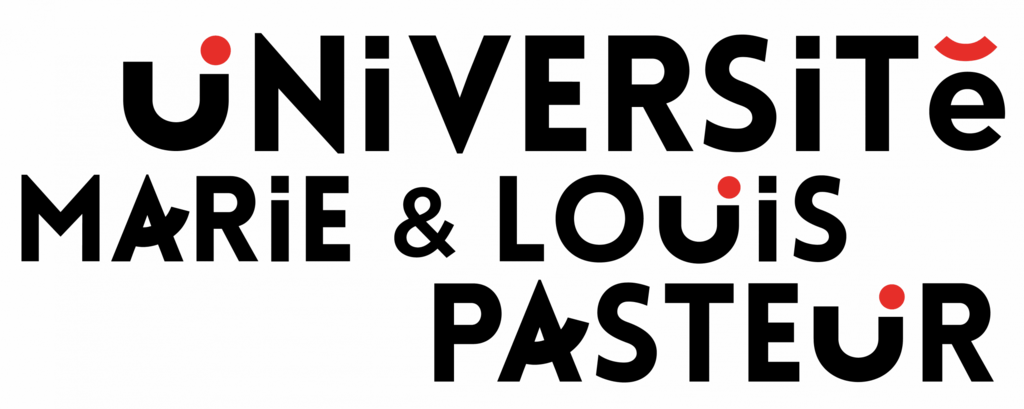
\includegraphics[height=25mm]{gfx/logo-UMLP.png}~\\[3cm]
    
    \textsc{\LARGE UFR Sciences et technique}\\
    \textsc{\Large Université Marie et Louis PASTEUR}\\
    \textsc{\Large \textbf{Projet}}\\
    \textsc{\Large L3 Informatique}\\[2.5cm]
    
    \HRule \\[0.4cm]
    { \huge \bfseries Jeu de plate-formes avec génération procédurale\\[0.4cm] } % C'est le titre donné par jube, j'y suis pour rien
    
    \HRule \\[0.6cm]\renewcommand\thesection{\arabic{section}}
    \textsc{\Large \textbf{Rapport de projet}}\\[1.5cm]
    \begin{minipage}{\textwidth}
      \begin{center}\LARGE
        Kilian \textsc{Jelic} \\
        Laura \textsc{Jacqueson} \\
        Théo \textsc{Pariney} \\
      \end{center}
    \end{minipage}
    \vfill
    % Bottom of the page
    {\large \ avril 2025}
    
  \end{center}
  %\end{sffamily}
\end{titlepage}

\normalsize
\pagenumbering{arabic}
\tableofcontents
\pagebreak
\listoffigures
\pagebreak

\section{Introduction}

Dans le cadre de notre projet semestriel en L3 Informatique à l'Université Marie et Louis Pasteur, nous avons travaillé sur le développement d’un jeu de plate-formes avec génération procédurale en C++. 

Les jeux de plate-formes sont un genre qui repose sur le contrôle d'un personnage avec des mécaniques comme les sauts et les obstacles, l’objectif étant généralement de rejoindre une sortie pour terminer le niveau. L’ajout de la génération procédurale introduit une caractéristique supplémentaire : plutôt que de concevoir chaque niveau à la main, un algorithme est chargé de créer les niveaux du jeu, permettant ainsi une expérience unique à chaque partie.

L'objectif principal de ce projet était de concevoir un jeu de plate-formes dont les niveaux seraient générés de manière procédurale, offrant ainsi une rejouabilité infinie. En parallèle, nous avons dû concevoir un jeu intégrant plusieurs mécaniques de jeu, incluant des déplacements, des sauts, un dash, ainsi qu’un objectif centré sur la récolte d’objets, tout en assurant la gestion des collisions et la physique du jeu.

Dans ce rapport, nous commencerons par une présentation générale du jeu, en exposant les objectifs du joueur et les scènes du jeu. Ensuite, nous détaillerons la conception des blocs et entités qui composent le monde et leur gestion dynamique. Par la suite, nous aborderons la génération procédurale, en expliquant la méthode utilisée ainsi que les détails d'implémentation. Nous discuterons ensuite des contrôles du personnage et des différentes mécaniques de jeu, telles que le saut, le dash, etc. La partie suivante sera consacrée à la physique, notamment la gestion des collisions et des propriétés physiques comme la résistance de l'air. Enfin, nous reviendrons sur l’organisation du travail, la répartition des tâches et les outils utilisés pour mener à bien ce projet. Le rapport se conclura par un bilan du projet et les améliorations possibles.

\pagebreak



\section{Présentation du jeu}
\subsection{Présentation générale}

Ce projet consiste à développer un jeu de plate-forme en 2D intégrant un système de génération procédurale de niveau. L’objectif est d’offrir une expérience où chaque partie est unique : au lieu d’avoir des niveaux prédéfinis, ceux-ci sont générés aléatoirement à chaque nouvelle partie. Contrairement aux jeux de plate-forme classiques où l'on peut apprendre les niveaux par cœur, ici, aucun parcours ne peut être rejoué à l’identique. Cette approche permet non seulement une rejouabilité infinie, mais aussi un défi constant, obligeant le joueur à s’adapter à chaque nouvelle configuration de niveau.

Le joueur incarne un petit robot, dont la mission principale est de récolter un maximum d’écrous avant d’atteindre la sortie du niveau. Ces écrous sont disposés aléatoirement dans l’environnement, incitant le joueur à explorer avant de pouvoir terminer la partie.

Pour évoluer dans le monde, le joueur dispose de plusieurs mécaniques lui permettant de se déplacer librement et d’interagir avec son environnement :
\begin{itemize}
  \item \textbf{déplacement} : le personnage peut se déplacer latéralement, à gauche et à droite, pour parcourir le niveau.
  \item \textbf{saut} : le personnage peut sauter pour franchir des obstacles ou atteindre des plateformes situées en hauteur.
  \item \textbf{double saut} : après un premier saut, lorsqu'il est encore en l’air, le personnage peut effectuer un second saut lui permettant d’atteindre des zones plus élevées.
  \item \textbf{dash} : le personnage dispose également d’un dash, une impulsion rapide dans une direction (gauche ou droite), utile pour traverser de grands espaces vides ou esquiver des obstacles.\\
\end{itemize}

Ces mécaniques offrent une grande liberté de mouvement, permettant aux joueurs d’adopter différentes stratégies. Certains privilégieront une approche prudente, optimisant chaque saut pour éviter la mort, tandis que d’autres tenteront des enchaînements rapides et fluides pour terminer le niveau efficacement.


Comme mentionné précédemment, tous les niveaux sont générés de manière procédurale, cela signifie qu'à chaque lancement de partie c'est un algorithme qui se charge de créer un environnement en plaçant des blocs, plateformes, échelles, écrous, piques et une sortie. Cette méthode permet de générer de manière presque infinie des mondes différents. 

Ces différent niveaux sont composés de salles générées de manière 
contiguës, et les salles sont reliées entre elles par des échelles et des
plateformes, de façon à ce que chaque niveau soit possible, en partant du
début jusqu'à la fin. Des blocs et plateformes de glace et de slime sont 
également générés, et le joueur doit donc faire attention aux changements 
que cela implique sur ses déplacements.
%ajout d'une petite présentation de l'algo de génération


\subsection{Les objectifs du joueur}

Dans ce jeu de plate-forme, le joueur incarne un petit robot dont l’objectif principal est de récupérer des écrous dispersés dans l’environnement avant d’atteindre la sortie.


\subsubsection{Les écrous}

Les écrous sont des objets collectables répartis à plusieurs endroits du niveau. Ils constituent un élément central du jeu, car ils encouragent le joueur à explorer le monde plutôt que de se précipiter vers la sortie.

Comme tous les autres éléments du monde, les écrous sont placés aléatoirement à chaque génération de niveau. Leur nombre n’est pas fixe, ce qui signifie que chaque partie offre une répartition différente des écrous, renforçant ainsi la rejouabilité. Le joueur doit donc parcourir l’environnement avec attention pour être sûr de ne pas en oublier.

Toutefois, la collecte des écrous n’est pas obligatoire pour terminer un niveau. Le joueur peut choisir de se concentrer sur la recherche de la sortie ou, au contraire, tenter de récupérer un maximum d’écrous pour améliorer son score, affiché dans le coin supérieur gauche de l’écran.


\subsubsection{La sortie}

La sortie représente l'objectif final d'une partie. Une fois que le joueur l'a trouvée, il peut choisir de l’atteindre immédiatement pour terminer la partie ou bien continuer à explorer afin de collecter davantage d’écrous et améliorer son score. Ce choix introduit un élément de stratégie, puisque le joueur doit évaluer s’il préfère sécuriser sa progression ou prendre des risques pour maximiser ses points.

Comme pour les écrous, la sortie est placée aléatoirement dans le niveau, ce qui signifie que le joueur ne sait jamais à l’avance où elle se trouve. Il est donc obligé d’explorer activement l’environnement pour la localiser.

Le fait que la sortie soit générée aléatoirement renforce la diversité des parties. Chaque session de jeu demande au joueur de s’adapter aux conditions spécifiques du niveau généré, ce qui augmente le défi et évite toute monotonie. Trouver la sortie peut parfois être simple, mais dans d’autres cas, elle pourra être bien cachée ou difficile d’accès, obligeant le joueur à parcourir l’intégralité du niveau.

Enfin, atteindre la sortie ne signifie pas nécessairement que le joueur a maximisé son score, mais cela valide sa progression et lui permet de lancer une nouvelle partie avec un niveau entièrement différent.



\subsection{Les scènes}


\section{Les blocks et entités du monde}
\subsection{La définition dynamique des blocks}
% Fichier XML et récupération dans une classe dédiée
\subsection{Le stockage des blocks}
% Récupération dans le blockmanager utilisé par le monde

\section{La génération procédurale}
% Je sais pas trop comment ça se passe, faudrait le remplir
% Faudra penser à préciser qu'on a commencé par faire un monde "test" avant d'arriver à notre générateur actuel
% Et aussi à donner les étapes/difficultés avant d'en arriver à un truc qui marche correctement

\subsection{Aléatoire et graine de génération}

À des fins de débuggage, la possibilité de pouvoir générer le même monde
plusieurs fois est importante. Pour cela, les niveaux sont générés à l'aide
d'un générateur de nombres pseudo-aléatoire. Ce générateur peut utiliser
un entier codé sur 64 bits, et générera la même séquence de nombres
aléatoires tant que la même graine est utilisée. 

Nous avons donc implémenté
deux moyens de générer les mondes: avec ou sans graine. Si une graine est
donnée au générateur, alors cette graine sera utilisée lors de la création
du niveau. Sinon, une graine aléatoire est choisie, et est affichée dans
la console. Cela permet, en cas de problème, de facilement noter et partager
une graine, permettant de reproduire le problème plus facilement.

\subsection{Étapes de génération}
\subsubsection{Génération des salles}

Les salles sont générées de manière à ce qu'elles soient connectées entre
elles, sans jamais se chevaucher. Pour cela, l'algorithme suivant est 
appliqué:

\begin{itemize}
  \item Générer une salle de départ.
  \item Tant que le nombre de salles voulu n'est pas atteint:
  \begin{itemize}
    \item Choisir aléatoirement la taille de la salle.
    \item Choisir une direction (haut, bas, gauche ou droite)
    \item Créer une nouvelle salle, placée à côté de la salle précédente,
    aléatoirement le long du mur correspondant à la direction choisie.
    \item Si la salle chevauche une autre salle, la regénérer.
    \item Si, au bout d'un certain nombre d'essais, la salle n'a pas réussi
    à se générer, réessayer en changeant la taille de la salle.
    \item Si la salle n'arrive toujours pas à se générer, supprimer la
    salle ainsi que la salle précédente, et regénérer la salle précédente.
  \end{itemize}
\end{itemize}

Certains cas spéciaux se présentent avec cet algorithme:
\begin{itemize}
  \item \textbf{La salle de départ}: La salle de départ, étant la première
  salle, ne peut pas se générer à la suite d'une autre salle. Elle se 
  génère donc simplement aux coordonnées (0, 0)
  \item \textbf{Retour en arrière}: Dans certains cas, une salle peut se 
  retrouver encerclée par d'autre salles. Dans ce cas, aucune salle ne 
  pourra se générer par la suite. Afin d'éviter ces situations, l'
  algorithme décide, si une salle n'arrive pas à se générer, de réessayer 
  d'abord avec une salle de différente taille, car une salle plus petite
  peut éventuellement réussir à se générer. Mais, au bout d'un certain 
  nombre d'essais, l'algorithme décide de retourner en arrière. Dans ce
  cas, la salle précédente est supprimée, et, en prenant un autre chemin,
  le générateur réussira à générer l'ensemble des salles.
  \item \textbf{Taille minimale d'entrée}: La génération de plateformes et 
  de pièges pourrait rendre l'entrée dans une salle impossible dans des cas
  où l'entrée d'une salle serait trop petite. Afin d'éviter cela,
  lorsqu'elles se placent le long d'un mur, les coordonnées aléatoires ont
  été restreintes afin que l'entrée vers la salle suivante aie toujours
  une taille minimale. Cette taille a été définie à 2 blocs. Dans la
  figure~\ref{fig:room_placement}, on peut voir que peu importe où se génère la
  salle, l'entrée de la salle verte vers la salle bleue aura toujours une
  taille d'au moins 2 blocs.
\end{itemize}

\begin{figure}[ht]
  \centering
  
\includegraphics[width=0.5\textwidth]{images/room_placement.png}
  \caption{Un exemple de placement de salle.}
  Une salle est représentée en vert.\\ 
  Si la direction haut est choisie, une salle de taille 3x3 peut\\
  se générer n'importe où dans la zone bleue.
  \label{fig:room_placement}
\end{figure}

Les salles étant une donnée réutilisée fréquemment par le générateur,
elles sont stockées en tant que liste de vecteurs contenant une position
x et y, ainsi que la taille de la salle (voir figure~\ref{fig:room_data}).

\begin{figure}
  \centering
  
\includegraphics[width=0.5\textwidth]{images/room_storage.png}
  \caption{Une représentation du stockage d'une salle, 
  en tant que coordonnée et taille de salle}
  \label{fig:room_data}
\end{figure}

\subsubsection{Génération des murs}

\subsubsection{Génération du chemin}

\subsubsection{Fausses plateformes et échelles}

\subsubsection{Placement des blocs spéciaux}

\subsubsection{Placement des pièges}

\subsubsection{Placement de la sortie}

\subsection{Monde de test}

Afin de tester des fonctionnalités du jeu comme les collisions, les 
échelles ou autres, un monde de test a été ajouté, sous la forme d'un 
générateur de monde. Dans le code, nous pouvons changer le générateur de
niveau en notre générateur de monde de test, et le monde généré sera alors
un monde simple, contenant une plateforme et autres fonctionnalités que
nous voulons tester (voir figure~\ref{fig:test_world}).

\begin{figure}[ht]
  \centering
  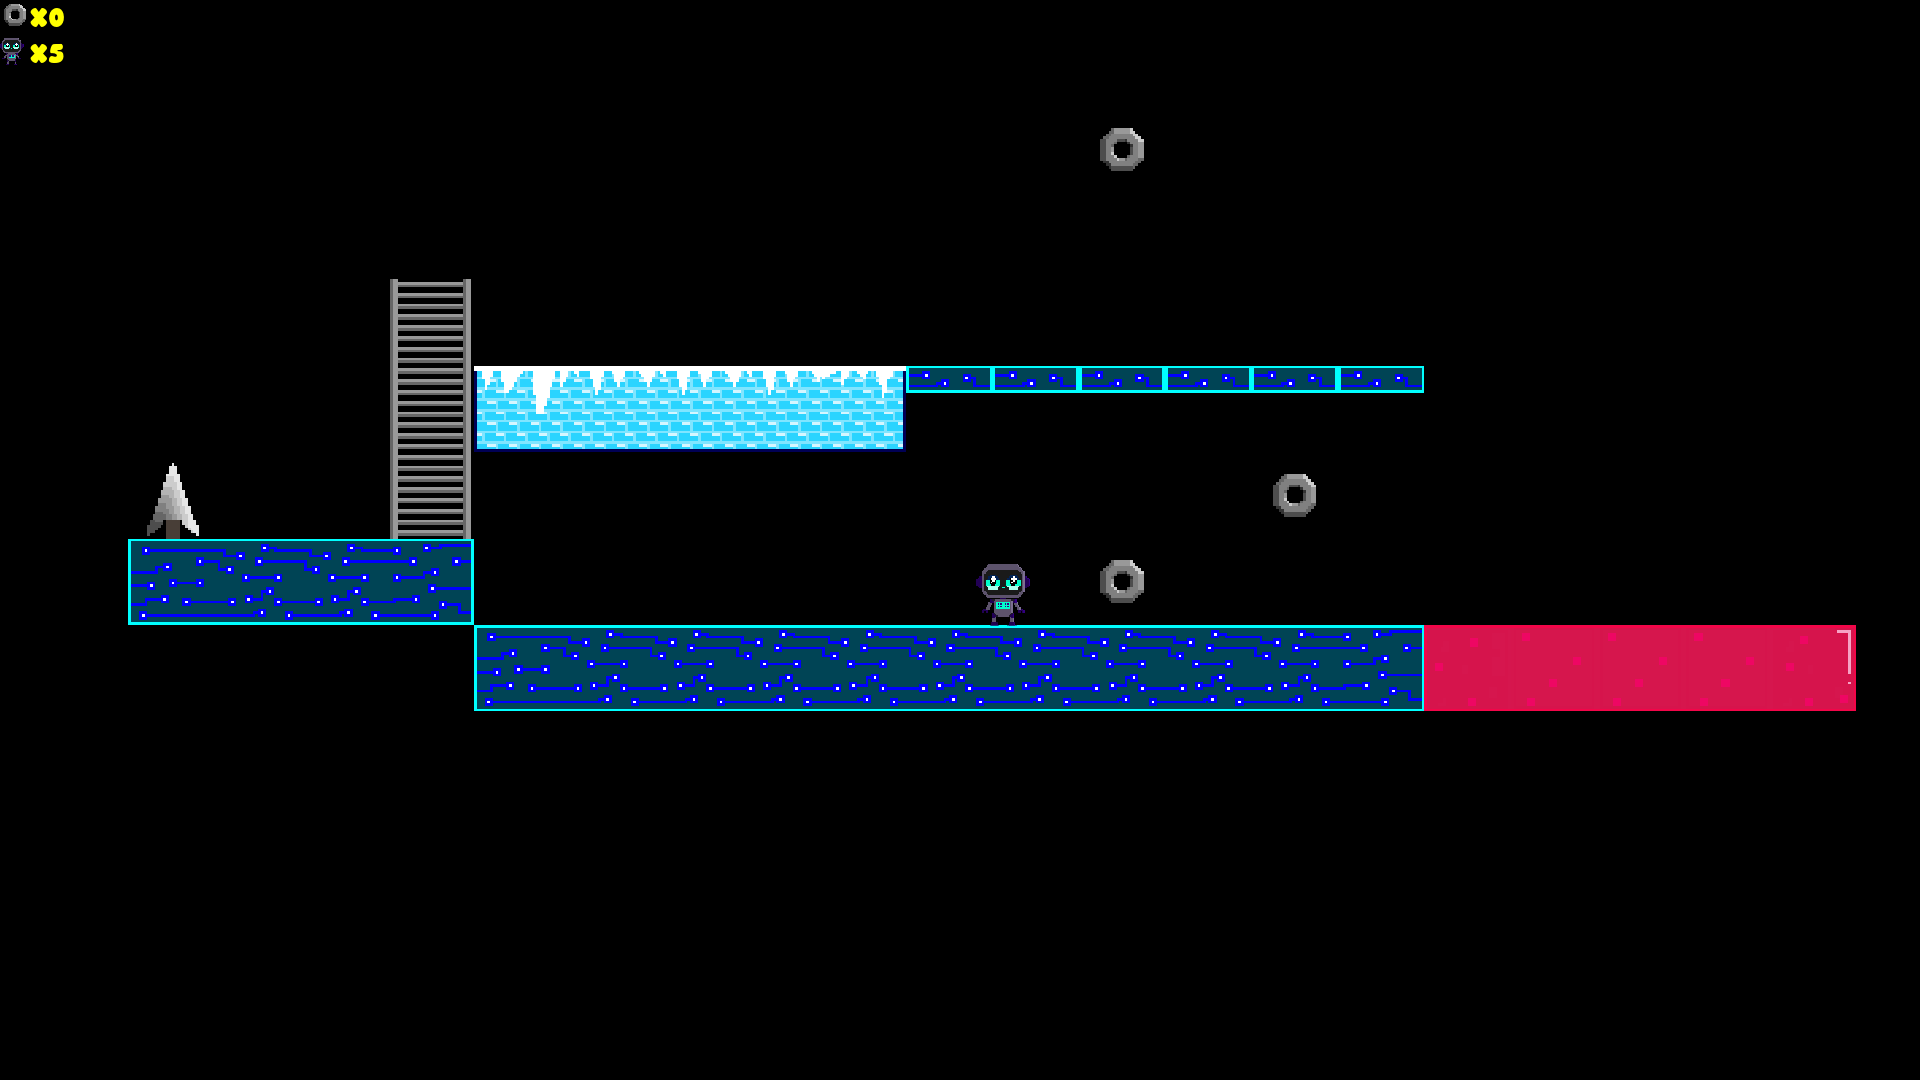
\includegraphics[width=\textwidth]{images/test_world.png}
  \caption{Une capture d'écran du monde de test}
  \label{fig:test_world}
\end{figure}

\section{Le personnage}
\subsection{Les contrôles de base}
\subsection{Le saut}
\subsubsection{Le saut modulable}
%ça fait partie des choix qu'on a fait puis abandonné, c'est important à mentionner
\subsubsection{Le double saut}
\subsection{Le dash}
%Faudra aussi mentionner qu'on a eu du mal à trouver des contrôles convenables
\subsection{Le score et les vies}

\section{La physique}
Lorsque nous avons commencé le projet, nous avions le choix entre réaliser la physique nous-même, et nous appuyer sur un moteur physique déjà existant.
En suivant les conseils de notre responsable de projet, nous avons finalement choisi d'implémenter notre propre moteur physique.\par

Nous avons pris la décision de réaliser une physique basée sur les impulsions.
Ainsi, les déplacements et les collisions sont calculées comme des vecteurs, qui sont ensuite appliqués aux divers éléments du jeu.\\
Pour cela, le moteur physique a pour tâche de pouvoir gérer :
\begin{itemize}
  \item[-] La détection de collisions entre le personnage et les éléments du décor
  \item[-] La résolution de ces collisions
  \item[-] La friction entre le personnage et le sol
  \item[-] La résistance de l'air, ralentissant la chute du personnage.
\end{itemize}

\subsection{La gestion des collisions}
La première étape de la réalisation du moteur physique a été la gestion des collisions.\\
Le seul élément de jeu pouvant se déplacer étant le personnage, les seules collisions à détecter et résoudre sont celles entre le personnage et les éléments du décor.\\
Nous avons choisi de représenter les éléments du décor et le personnage par des formes rectangulaires, ce qui simplifie la tâche, les collisions rectangle-rectangle étant les plus simples à calculer.
De plus, le décor étant stocké sur une grille de blocks de même taille, seuls les blocs se trouvant dans les cases adjacentes à celle où se trouve le personnage joueur sont susceptibles d'entrer en collision avec lui, ce qui implique qu'à n'importe quel instant, il n'est nécessaire de tester les collisions qu'avec 9 cases :
les 8 entourant le joueur et celle sur laquelle il se trouve.\par

La détection des collisions n'a pas été un problème, celle si étant gérée par la classe \emph{collide} de gamedev framework.\\
La première difficulté que nous avons rencontré a été lors de la résolution des collisions, ceci restant une étape complexe dans la création d'un moteur physique même lorsqu'uniquement des rectangles sont impliqués.\par

Une fois une collision détectée entre un bloc du décor et le joueur, on commence par déterminer la vélocité relative \(V\) entre les éléments.
Étant donné que le block est immobile, cette vélocité est donnée par :
\[ V =  - V_{P} \]
Où \(V_{P}\) est la vitesse du joueur.\\
Une fois cette vitesse déterminée, on peut l'utiliser pour calculer la vitesse \(V_{n}\) par rapport à la normale de collision \(n\), donnée par la détection de collisions de gamedev framework :
\[ V_{n} = V \cdot n \]
Si \(V_{n}\) est négative, cela signifie que le joueur ne se déplace pas en direction du bloc, et la collision n'a pas à être résolue.\\
Cette vitesse nous permet de calculer la magnitude de l'impulsion \(C_{i}\) à appliquer au joueur :\\
\[ C_{i} = (1 + e) \times V_{n} \]
Où e est le \emph{coefficient de restitution} du bloc avec lequel le joueur est entré en collision.\\
Ce coefficient permet de déterminer la puissance du "rebond" que le joueur subira après avoir quitté le bloc.\\
Dans un moteur physique classique, il serait nécessaire de prendre en compte le coefficient de restitution des deux entités entrant en collision, mais le joueur étant le seul élément entrant en collision, nous avons simplifié le modèle en ne prenant que celui du bloc.\\
Finalement, nous pouvons calculer le vecteur de résolution de collision \(V_{res}\) à appliquer au joueur :
\[V_{res} = C_{i} \times n \]

\subsection{Correction positionnelle}
Dans le modèle que nous avons choisi, chacun des objets possède une masse infinie, ce qui explique qu'elle n'apparaisse pas dans les calculs. Cependant, les imprécisions causées par les flottants amènent le joueur à s'enfoncer dans les blocs lorsqu'il est immobile dessus.\\
Pour résoudre cela, nous pouvons appliquer en plus du vecteur de résolution de collision, un second vecteur de correction positionnel \(V_{corr}\) donné par :
\[V_{corr} = -max(d-0.1,0) \times C_{corr} \times n\]
Avec :\\
\begin{itemize}
  \item[-] \emph{d} : La profondeur de collision, c'est-à-dire la distance dans laquelle le joueur s'est enfoncé dans le bloc
  \item[-] \(C_{corr}\) : Le coefficient de correction, indiquant la force de correction qu'il est nécessaire d'appliquer. Nous avons choisi d'avoir \(C_{corr}=0.8\)
\end{itemize}

\subsection{Resolution de la friction}
Le moteur physique doit ensuite être capable de gérer la friction que le personnage pourra subir en se déplaçant sur les blocs au sol.\\
Pour cela, on commence par recalculer la vélocité relative du joueur \(V\) par rapport au bloc après l'application de \(V_{res}\) :
\[V =  - (V_{P} + V_{corr})\]
Cette fois, nous avons besoin de la tangente \(t\) pour connaître la direction sur laquelle appliquer la friction, qu'on peut déterminer par :
\[t = V - relativeVelocity \cdot (n \times (1,0)) \times n\]
Une fois la tangente connue, il est possible de calculer le coefficient de friction \(C_{f}\), correspondant à la vélocité relative à la tangente :
\[C_{f} = - V \dot t\]
D'après la loi de Coulomb sur la friction, la force de friction est toujours inferieure à la force normale multipliée par le coefficient de friction statique \(\mu_{s}\) des materiaux entrant en friction. Nous pouvons donc déterminer le vecteur de friction \(C_{f}\) à appliquer grâce à l'équation :
\[
V_{f} = \left\{\begin{array}{lr}
           C_{f} \times t & \text{si } |C_{f}| < |C_{i}| \times \mu_{s}\\
          -C_{i} \times t * \mu_{d} & \text{si } |C_{f}| \geq |C_{i}| \times \mu_{s}
        \end{array}\right\}
\]
Où \(\mu_{s}\) et \(\mu_{d}\) sont respectivement le coefficient de friction statique et dynamique du block avec lequel le joueur entrant en friction.

\subsection{Collisions avec des platformes directionnelles}
En plus des blocks classiques, nous avons fait le choix d'ajouter des platformes directionnelles, à travers lesquelles le joueur passe à moins de venir d'une direction particulière.\\
Leur particularité implique l'implémentation de caractéristiques supplémentaires lors de la détection et la résolution de collisions.\\
Premièrement, une fois la collision détectée, on teste la direction de mouvement du joueur par rapport à la normale de collision, donnée par :
\[
  angle(n,Dir_{block}) + \pi
\]
Où \(Dir_{block}\) correspond à un vecteur donnant la direction attendue du joueur pour avoir une collision (\((0,-1)\) pour un block orienté vers le haut), et \(angle\) une fonction retournant l'angle entre 2 vecteurs.\\
Si cet angle est superieur à un seuil, que nous avons choisi comme étant \(0.1\), alors on considère que le joueur ne se trouve pas dans la bonne direction, et la collision n'a pas lieu.\par
Secondement, dans le but d'éviter que la collision soit résolue dans le cas où le joueur soit en train de tomber à travers la platforme, la collision est détectée avec des hitbox de taille réduite, orientées dans la direction de la collision. Ainsi, pour les collisions entre entre une platforme orientée vers le haut, le joueur et la platforme disposent d'une hitbox d'un huitième de bloc, respectivement placée en haut et en bas des hitbox classiques.\par
Ces deux algorithmes ne permettent pas de complètement effacer le problème, mais celui-ci est suffisemment réduit pour n'être que rarement visible.

\subsection{Collisions multiples}
Lorsque le joueur entre en collisions avec de multiples blocs, le vecteur de résolution de collision, de correction ainsi que le vecteur de friction résultants correspondent à la moyenne des vecteurs obtenus en résolvant les collisions, corrections et frictions avec les blocks.

\subsection{Stockage des données de collision}
L'ensemble des données est stocké et retourné dans une structure dédiée, permettant de conserver :

\begin{itemize}
  \item La moyenne des vecteurs obtenus par la résolution de collision, correction et friction
  \item Des booléens indiquant s'il est nécessaire d'appliquer le vecteur de résolution de collision ou la correction
  \item L'ensemble des types de blocs avec lesquels une collision est survenue, qu'elle ait été résolue ou non (ce qui permet de détecter les collisions avec les piques ou les écrous)
  \item L'ensemble des coordonnées des blocs avec lesquels une collision est survenue, résolue ou non (ce qui permet notemment l'effacement des écrous de la grille)
\end{itemize}

Cette structure est ensuite transmise au personnage, qui pourra appliquer les vecteurs de résolution de friction et de collision à sa vitesse, et corriger sa position.

\subsection{Résistance de l'air}
La résistance de l'air permet de réduire l'accéleration du joueur lors de sa chute, en fonction de sa vitesse actuelle.\\
Nous avons choisi de l'implémenter afin d'avoir plus de mobilité en l'air, et d'éviter au joueur d'atteindre des vitesses énormes trop vite en chutant.\\
La résistance de l'air est calculée dans une fonction séparée, et est donnée par :
\[
 -dir \times v^2
\]
Où \(dir\) est la direction du joueur, et \(v\) sa vitesse actuelle.

\section{Notre organisation}
\subsection{La définition des tâches}
\subsubsection{La répartition du travail}
\subsection{Les outils utilisés}
% ça serait important de mentionner qu'on a mis un peu de temps à avoir un trello
% je pense aussi que l'ordre dans lequel on a mis les outils en place peut être interessant à rajouter
\subsubsection{GameDev Framework}
% Il faut quand même mentionner notre cher Jube pour son joli framework
\subsubsection{Discord}
\subsubsection{Google Docs} %Pour les idées à la base
\subsubsection{Trello}
\subsubsection{Git et Github}
\subsubsection{IDE}
% Cette section là elle est marrante parce que personne utilise le même
\newpage

\section{Conclusion}
% On a quand même une conclusion ici avant les autres points
\subsection{Points d'amélioration}
\subsubsection{Ce qu'on aurait voulu ajouter}
%c.f le gdoc
\subsubsection{Wave Function Collapse}
\subsubsection{Pathfinding amélioré}
\subsubsection{La physique} % ;-;


\end{document}
